\chapter{Vlastní přístup}

V této kapitole navrhnu vlastní inovativní přístup k dynamicky vyvažované obtížnosti. Mnou navržené algoritmy vychází z již existujících algoritmů teorie her a z tohoto důvodu se v první sekci této kapitoly věnuji základům z teorie her a popisu algoritmů, jež jsem převzal a upravil pro využití v DDA. V druhé sekci se již věnuji popisu vlastních algoritmů.

\section{Teorie her}

S teorií her se lze setkat především v ekonomické oblasti. Pro tuto sekci jsem vybral pouze témata z teorie her, jež budou využity. Nejdříve neformálně zadefinuji různé druhy her, hry v extenzivní formě a zero-sum hry. Následně nastíním algoritmy Minimax a Monte Carlo prohledávání stromu, které se používají pro hráče her v extenzivní formě.

\subsection{Základní definice}

\subsubsection{Dělení her}

Hry můžeme dělit dle obsahu nedeterminismu nebo dle úplnosti informace. U deterministických her je stav hry určen pouze rozhodnutím hráčů. Naopak u nedeterministických her je stav hry určen kombinací rozhodnutí hráče a projevu náhody. Mezi deterministické hry patří např. dáma a šachy. Naopak k nedeterministickým hrám se např. řadí hry využívající hrací kostku jako je Člověče, nezlob se.

Dle úplnosti informace dělíme hry na hry s úplnou a neúplnou informací. U her s úplnou informací všichni hráči znají kompletní stav hry a žádná informace jim není skryta. Naopak u her s neúplnou informací existuje část stavu neznámá všem hráčům. Mezi hry s neúplnou informací patří většina karetních her, kdy hráči neznají karty v soupeřově ruce.

\begin{table*}[b]\footnotesize
\vspace*{0mm}
\caption{{\label{tab:klasifikaceher}} Klasifikace her dle úplnosti informace a determinismu.}
\vspace*{0mm}
\label{shadowtable}
\begin{center}
\begin{tabular}{ l || l | l |}
 & S úplnou informací & S neúplnou informací \\
\hline
\hline
Deterministické & šachy, dáma & Hledač min \\ \hline
Nedeterministické  & Člověče, nezlob se & Prší \\ \hline
\end{tabular}
\end{center}
\end{table*}

\subsubsection{Extenzivní forma hry}

Hry v teorii her můžou být znázorněny ve dvou základních formách - normální a extenzivní forma. Hry v normální formě jsou používány pro hry, kde se hráči rozhodují současně. My budeme potřebovat formu vhodnou pro hry, kde se hráči ve svých rozhodnutích střídají a kde se rozhodují na základě dřívějších rozhodnutích. Průběh takové hry můžeme znázornit pomocí grafu. Tento graf se nazývá herním stromem. Graf je orientovaný s jedním kořenem a je bez cyklů. Uzly stromu představují možné stavy hry. Stav hry mimo jiné obsahuje informaci o hráči, který je na řadě. Hrany vedoucí z uzlu odpovídají všem možným tahům hráče, který je v daném stavu na řadě. Kořen představuje počáteční stav hry a listy stavy koncové. Všechny listy mají přiřazenou utilitu/zisk pro každého hráče. Jednoduchá utility funkce přiřadí hodnotu +1 výherci a -1 všem ostatním hráčům, v případě remízy přiřadí 0 všem hráčům.

Příklad herního stromu varianty piškvorek 3x3 Tic-Tac-Toe jen na Obr. \ref{fig-ttt-minimax}. V této hře se hráči pravidelně střídají, a proto uzly ve stejné hloubce odpovídají tahům stejného hráče. Aktuální hráč je v obrázku znázorněn vlevo. Ve spodní části jsou ukázány listy s utilitou pro hráče hrajícího křížky.

\begin{figure}
  \centering
  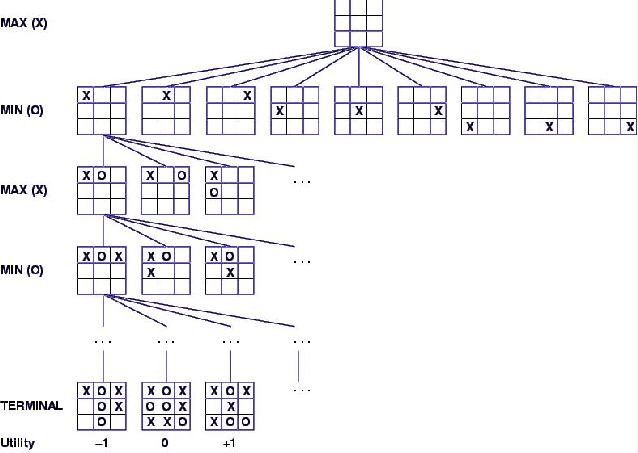
\includegraphics[width=0.75\textwidth]{ttt-minimax}
	\caption{ Výřez herního stromu hry Tic-Tac-Toe. }
	\label{fig-ttt-minimax}
\end{figure}

U nedeterministických her existují vnitřní uzly dvou typů. První odpovídá tahu aktuálního hráče stejně jako u her deterministických. Druhým typem je uzel náhody (chance node). Uzel náhody odpovídá stavu hry, kdy je na řadě náhodná událost - např. hod kostkou. Hrany z tohoto uzlu odpovídají náhodným jevům, možným stavům hry po náhodné události. Hrany jsou navíc ohodnocené číslem, které představuje pravděpodobnost jednotlivých náhodných jevů. V případě hodu kostkou budou všechny hrany ohodnoceny $\frac{1}{6}$.

U her s neúplnou informací hráči přesně nevědí, v jakém konkrétním uzlu herního stromu se nacházejí. Z jejich pohledu může být více uzlů představovat aktuální stav hry. Tato množina navzájem od sebe nerozlišitelných uzlů se nazývá informační množinou. Přestože hráč přesně neví, v kterém uzlu v rámci informačního stromu se nachází, může přiřazovat různé pravděpodobnosti jednotlivým stavům na základě předchozích tahů soupeřů.

Herní strom můžeme upravit pro hry s neúplnou informací. Uzel takového stromu nemusí představovat pouze jeden stav hry, ale celou množinu stavů, odpovídající informační množinu.

\subsubsection{Zero-sum hry}

Podkategorii her tvoří zero-sum hry. U těchto her platí, že součet utilit pro všechny hráče v každém listu se rovná 0. Tuto vlastnost využívají některé algoritmy, mezi které patří Minimax s alfa, beta prořezáváním.

U dvouhráčových zero-sum her můžeme pracovat pouze s utilitou pro jednoho hráče, utilita druhého hráče se snadno odvodí. Příkladem zero-sum hry je Tic-Tac-Toe. Z tohoto důvodu byla v herním stromu na Obr. \ref{fig-ttt-minimax} ukázána utilita pouze jednoho hráče.

\subsection{Algoritmy používané pro hry}

Existuje celá řada algoritmů umělé inteligence pro hry v extenzivní formě. V této podsekci popíši základní algoritmy Minimax s prořezáváním a Monte-Carlo prohledávání stromu, na jejichž základě navrhnu vlastní algoritmy pro DDA.

\subsubsection{Minimax}

V základní formě algoritmus Minimax pracuje pouze s dvouhráčovými zero-sum hrami. Každý z hráčů se snaží maximalizovat svojí utilitu a zároveň ví, že jeho soupeř se snaží jeho utilitu minimalizovat a tím maximalizovat utilitu svojí. 

Algoritmus prochází herní strom do hloubky až do listů. Ve chvíli, kdy získá vnitřní uzel utilitu ze všech potomků, vybere z utilit tu nejmenší/největší, kterou propaguje o patro výše. V soupeřově uzlu hráč vybírá minimum z potomků, ve svém uzlu vybírá maximum z potomků. Ve chvíli, kdy se dopropagují utility ze všech potomků ke kořeni, hráč vybere tah, který odpovídá uzlu s největší utilitou.

Ne vždy je možné procházet celý herní strom až do jeho listů. Často se omezuje maximální hloubka procházeného stromu. Jestliže algoritmus skončí v uzlu, který není listem, musí ohodnotit stav hry pomocí heuristické funkce a propagovat výše pouze odhadnutou utilitu. Heuristické funkce bývají herně specifické. Např. u hry dáma může být odhadnutá utilita rozdíl počtu zbývajících herních kamenů obou hráčů.

Rozšířenou variantou pro vícehráčové a ne nutně zero-sum hry je algoritmus MaxN. U těchto her se v listech stromu nenachází pouze jedna hodnota, ale každý hráč zde má svojí utilitu. Oproti základní verzi se zde propaguje výše celá skupina utilit. Každý hráč ve svém uzlu maximalizuje svojí utilitu.

\subsubsection{Alfa-beta prořezávání}

Alfa-beta prořezávání slouží k urychlení základního algoritmu Minimax aniž by to ovlivnilo jeho chování. Urychlení spočítá v prořezávání, neprocházení větví stromu, u kterých je již zřejmé, že nemohou obsahovat lepší tah pro aktuálního hráče v daném uzlu.

K ořezávání se používají proměnné alfa a beta. Alfa představuje maximální spodní hranici a beta naopak minimální horní hranici pro utilitu řešení v dané větvi herního stromu. V průběhu algoritmu se alfa může zvětšovat a beta naopak zmenšovat. Ve chvíli, kdy se překříží, si můžeme být jisti, že další expandování uzlu nepovede k řešení a další potomky neprocházíme.

Zrychlení algoritmu je silně závislé na pořadí procházení jednotlivých uzlů. Může výpočet až dvakrát zrychlit, ale může se stát, že se výpočet vůbec nezrychlí.

\subsubsection{Monte-Carlo prohledání stromu}

Jiným přístupem k vytvoření hráče je metoda Monte-Carlo prohledávání stromu. Oproti Minimaxu nepracuje s hotovým herním stromem. Herní strom si vytváří ve svém průběhu. Na začátku je herní strom tvořen pouze kořenem představující aktuální stav hry. Poté algoritmus v iteracích opakuje 4 kroky - selekce, expanze, simulace a zpětná propagace. 

Během \emph{selekce} se vybere list z částečně postaveného stromu. Při výběru se začne v kořeni a podle předem daného pravidla se volí potomci až se algoritmus dostane do listu. Vybraný list se \emph{expanduje}. Z listu se stane vnitřní uzel, přidají se mu potomci odpovídající možným tahům z daného stavu. Z každého přidaného uzlu se provede \emph{simulace} hry ideálně až do konce. Je nutné, aby simulace nebyla výpočetně náročná. Z tohoto důvodu se hráči volí tahy náhodně. Nakonec se výsledek hry \emph{propaguje} přes rodiče až do kořene.

\begin{figure}
  \centering
  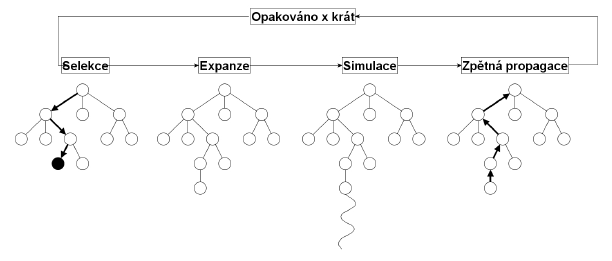
\includegraphics[width=0.75\textwidth]{ch4mcts}
	\caption{ Schéma jedné iterace MCTS. }
	\label{fig-ch4mcts}
\end{figure}

Každý uzel stromu obsahuje stav hry, aktuální aproximovanou hodnotu hry a počet navštívení uzlu během fáze selekce. 

Pravidlo pro selekci potomků není předem dáno. Jednou z často používaných metod selekce je UCT (Upper
Confidence bounds applied to Trees). Tato metoda se snaží vhodně vyvážit procházení slibných větví (s vysokou aktuální hodnotou) a procházení doposud málo navštívených uzlů. Každý z potomků je ohodnocen následujícím vzorcem:

	\[
	d_i = v_i + C * \sqrt{\frac{ln N}{n_i}}
\]

Poté se vybere uzel s největší hodnotou $d_i$ a proces se opakuje. Ve vzorci $v_i$ značí aktuální hodnotu i-tého potomka, $n_i$ počet navštívení potomka, $N$ počet navštívení rodiče. Pomocí konstanty $C$ se volí, jestli bude upřednostňováno procházení málo navštívených uzlů, nebo uzlů s vysokou hodnotou $v_i$. 

Volba počtu iterací je na programátorovi. Čím více iterací zvolí, tím lepšího chování dosáhne na úkor výpočetního času. Počet iterací nemusí být předem znám. Programátor se může rozhodnout pro ukončení algoritmu po určitém čase. Algoritmus má od konce první iterace vždy nějaké řešení, tah, který hráč má zvolit. Opakování iterací toto řešení zlepšuje.

\section{Hráč prostředí}



\subsection{E-HillClimber}

\subsection{Druhy}

\subsection{Treti}

\endinput
%%
%% End of file `ch01.tex'.
